% "{'classe':('PSI'),'chapitre':'dyn_pfd_co','type':('application'),'titre':'Wheeling moto', 'source':'Équipe PT - La Martinière Monplaisir','comp':('C1-05','C2-09'),'corrige':False}"
%\setchapterimage{bandeau}
\chapter*{Application \arabic{cptApplication} \\ 
Chaîne ouverte -- Wheeling moto\ifnormal $\star$ \else \fi \ifdifficile $\star\star$ \else \fi \iftdifficile $\star\star\star$ \else \fi
-- \ifprof Corrigé \else Sujet \fi}
\addcontentsline{toc}{section}{Application \arabic{cptApplication} : 
Chaîne ouverte -- Wheeling moto\ifnormal $\star$ \else \fi \ifdifficile $\star\star$ \else \fi \iftdifficile $\star\star\star$ \else \fi
-- \ifprof Corrigé \else Sujet \fi}

\iflivret \stepcounter{cptApplication} \else
\ifprof  \stepcounter{cptApplication} \else \fi
\fi

\setcounter{question}{0}
\marginnote{Équipe PT - La Martinière Monplaisir.}
\marginnote[1cm]{
\UPSTIcompetence[2]{C1-05}
\UPSTIcompetence[2]{C2-09}
}
\begin{marginfigure}
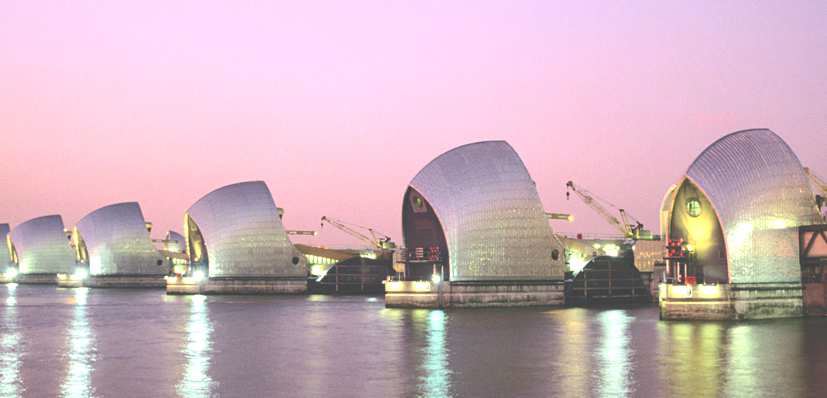
\includegraphics[width=\linewidth]{fig_00}
\end{marginfigure}


\subsection*{Modélisation}
L'étude proposée concerne l'étude dynamique d'une moto dans une phase de wheeling. Il s’agit d’une figure acrobatique consistant à soulever la roue avant, et de ne garder que l’appui sous la roue arrière. La moto est supposée se déplacer en ligne droite, sur une route horizontale, et l'étude menée est cinématiquement plane. Le modèle d'étude est sur la figure ci-dessous.

\begin{marginfigure}
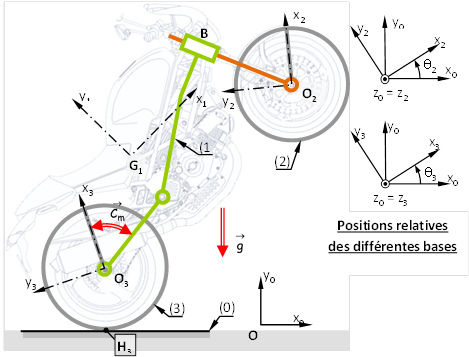
\includegraphics[width=\linewidth]{fig_01}
\end{marginfigure}

\begin{itemize}
\item $\mathcal{R}_0=\repere{O_0}{x_0}{y_0}{z_0}$ est un repère supposé galiléen, où $\vect{x_0}$ est dirigé suivant la vitesse de la moto et $\vect{y_0}$ suivant la verticale ascendante;
\item $\mathcal{R}_1=\repere{G_1}{x_1}{y_1}{z_1}$ est un repère lié à l'ensemble considéré indéformable \{cadre + bras arrière + fourche avant + pilote\}. On note $\theta_1=\angl{x_0}{x_1}$;
\item $\mathcal{R}_2=\repere{O_2}{x_2}{y_2}{z_2}$ est un repère lié à la roue avant (2), de rayon $R$ et de centre $O_2$ tel que $\vect{z_2}=\vect{z_0}$. On note $\theta_2=\angl{x_0}{x_2}$;
\item $\mathcal{R}_3=\repere{O_3}{x_3}{y_3}{z_3}$ est un repère lié à la roue arrière (3), de rayon $R$ et de centre $O_3$ tel que $\vect{z_3}=\vect{z_0}$. On note $\theta_3=\angl{x_0}{x_3}$. Les contacts entre les roues \textbf{(2)} et \textbf{(3)} et le sol \textbf{(0)} sont modélisés par des liaisons ponctuelles en $H_2$ et $H_3$.
\end{itemize}

\begin{marginfigure}
On note :
\begin{itemize}
\item $\vect{OO_3} = \lambda \vect{x_0}+R\vect{y_0}$;
\item $\vect{O_3O_2} = L_1\vect{x_1}$;
\item $\vect{O_3G_1} = a_1\vect{x_1}+b_1\vect{y_1}$;
\item $\vect{H_3O_3} = R \vect{y_0}$;
\item $\vect{H_2O_2} = R \vect{y_0}$;
\item $G_2 = O_2$ et $G_3 = O_3$.
\end{itemize}
\end{marginfigure}

On note $G_i$ le centre d'inertie, $m_i$ la masse et $C_i$ le moment d'inertie par rapport à l'axe   de la pièce \textbf{(i)}. 
\textbf{On fait l'hypothèse que le problème est plan.}
\subsection*{Étude dynamique}
La transmission exerce sur la roue arrière un couple moteur $\vect{C_m}=C_m\vect{z_0}$. 
On suppose que l’adhérence roue/sol est suffisante pour assurer le roulement sans glissement de la roue \textbf{(3)} au contact en $H$ avec le sol.
La situation initiale est définie au moment où la roue avant quitte le contact avec le sol, avec   $\dot{\theta_1}=0$ (après $\neq 0$).

\question{Construire le graphe de structure de la moto dans la phase de wheeling.
Préciser le degré de mobilité de l'ensemble, compte tenu de l'hypothèse de roulement sans glissement en $H_3$.}
\ifprof
\begin{corrige}
\end{corrige}
\else
\fi

\question{En se limitant à l'application des théorèmes généraux de la dynamique, définir quelles équations permettent de déterminer l'ensemble des équations de mouvement, en précisant:
\begin{itemize}
\item élément(s) isolé(s) ;
\item théorème appliqué, en précisant quelle projection et quel point de réduction éventuel sont retenus. 
\end{itemize}
}

\ifprof
\begin{corrige}
\end{corrige}
\else
\fi


\question{Mettre en place les équations précédentes.
Conclure sur la possibilité d'intégration de ces équations. }
\ifprof
\begin{corrige}
\end{corrige}
\else
\fi



\ifprof
\else
\begin{marginfigure}
\centering

\includegraphics[width=3cm]{Cy_04_03_PFD_CO_App_01_MotoWheeling_qr}
\end{marginfigure}
\fi


\ifprof
\begin{center}
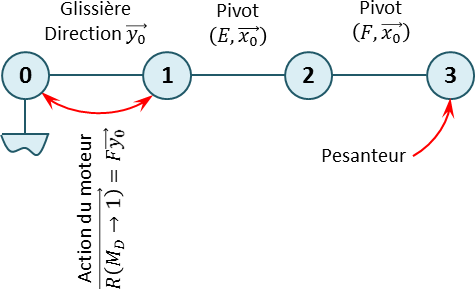
\includegraphics[width=.8\linewidth]{cor_01}
\end{center}

\begin{center}
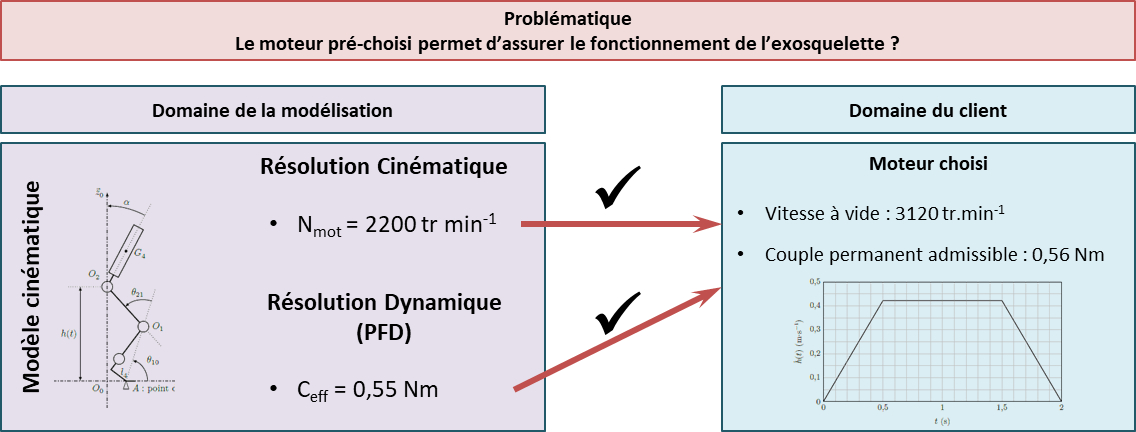
\includegraphics[width=\linewidth]{cor_02}
\end{center}

\begin{center}
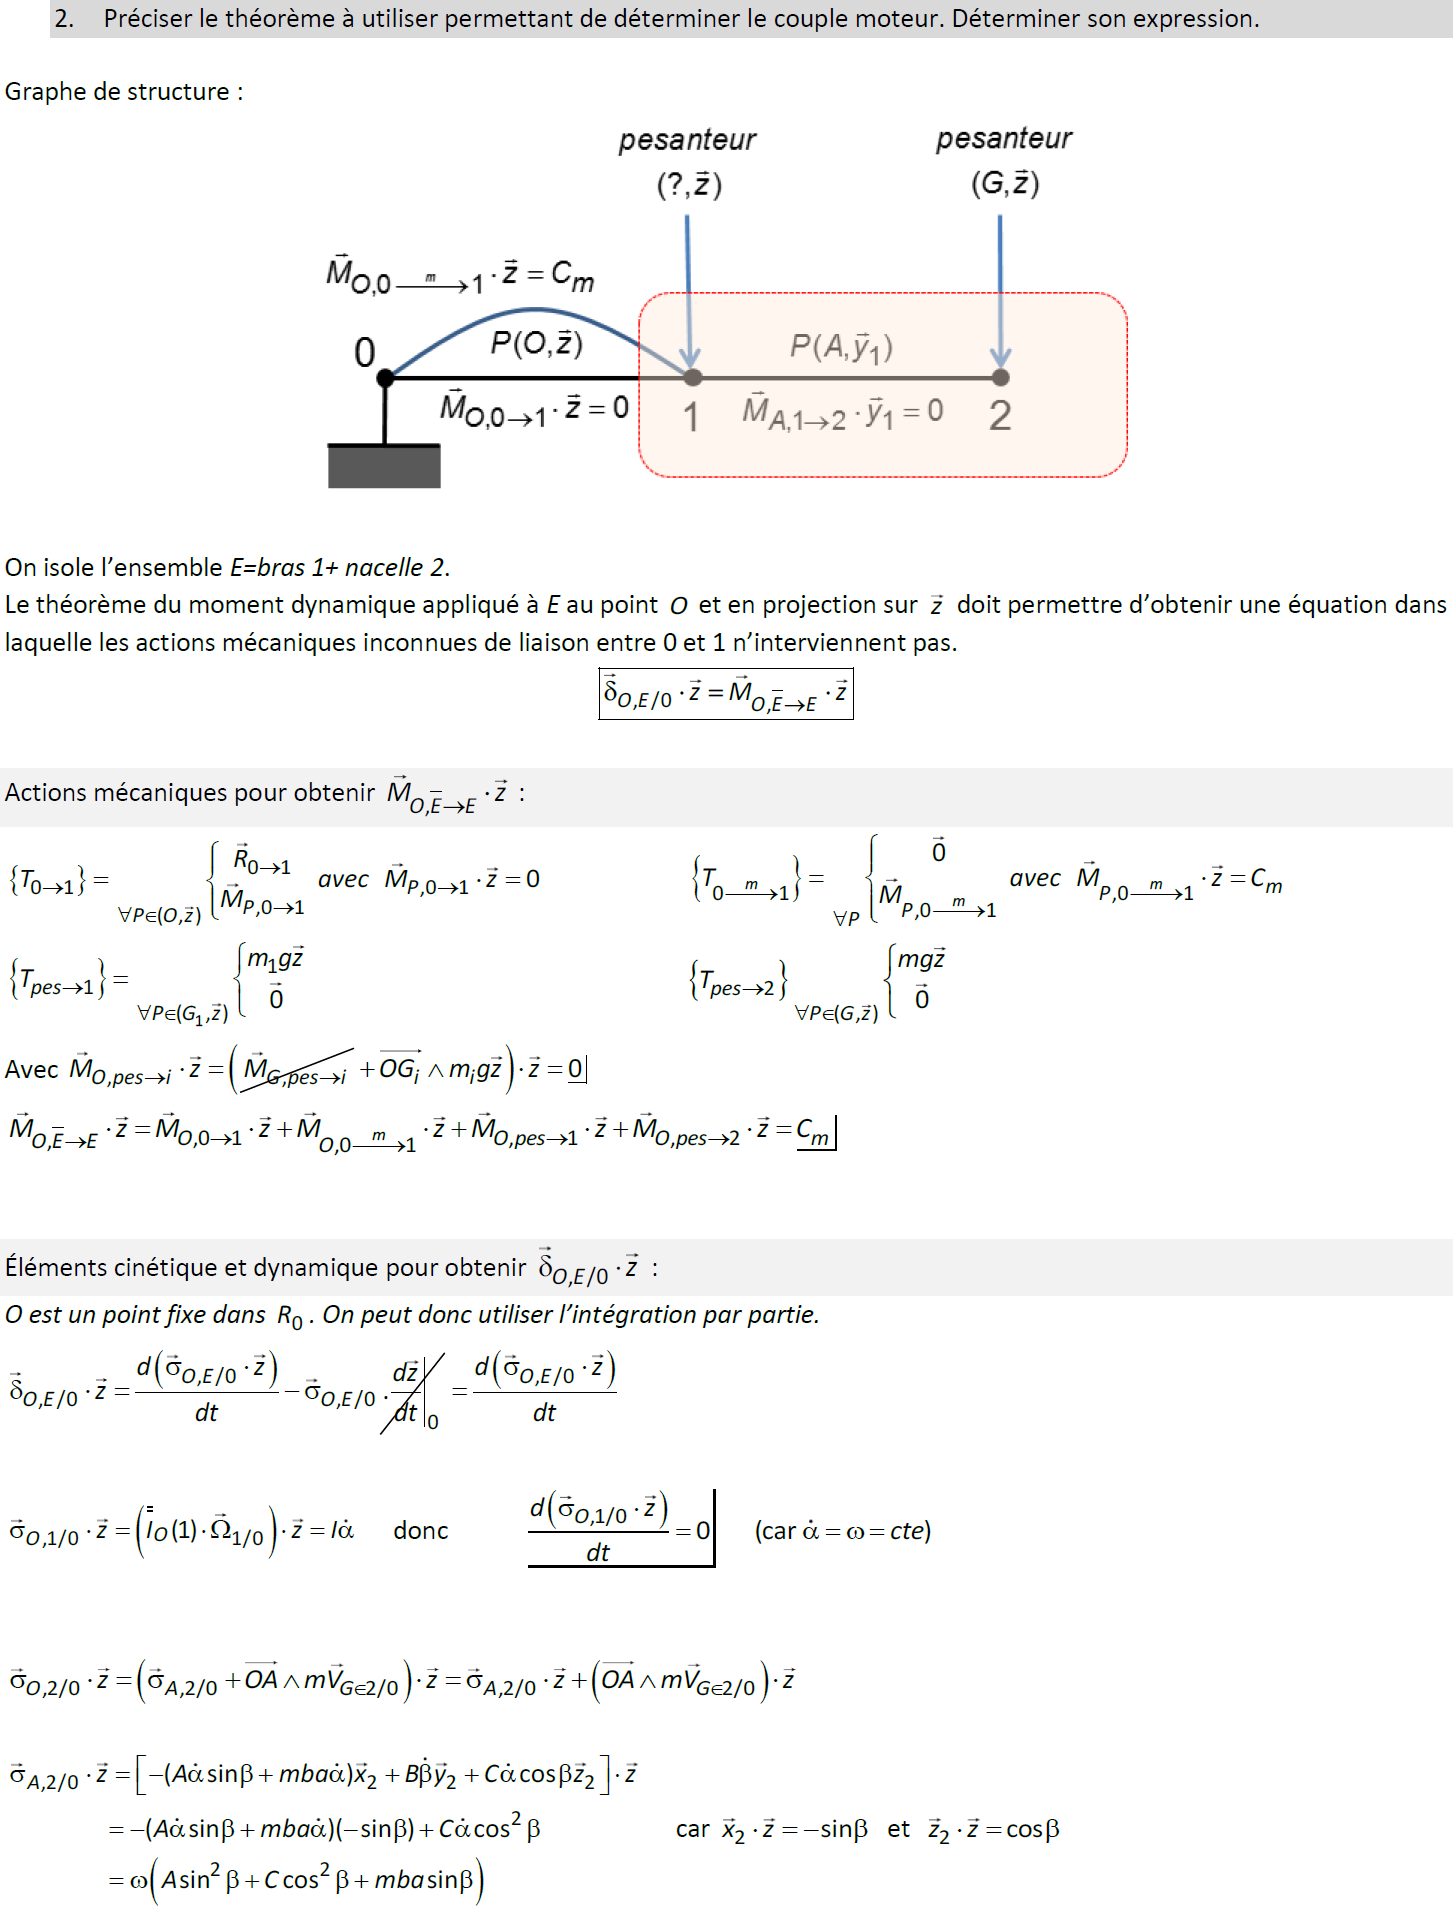
\includegraphics[width=\linewidth]{cor_03}
\end{center}

\begin{center}
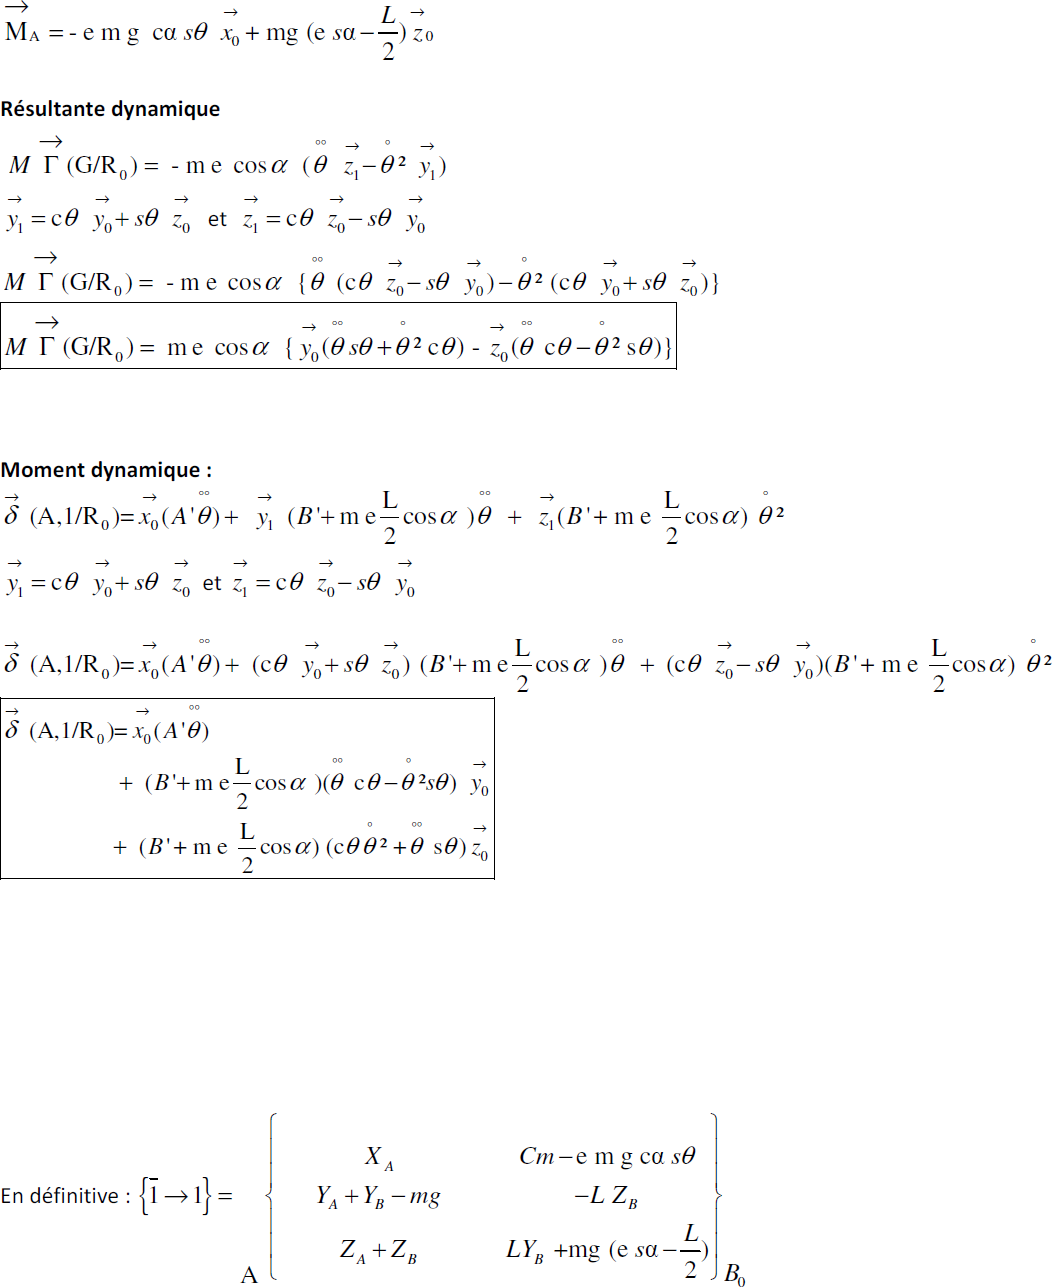
\includegraphics[width=\linewidth]{cor_04}
\end{center}
\else
\fi
%\begin{center}
%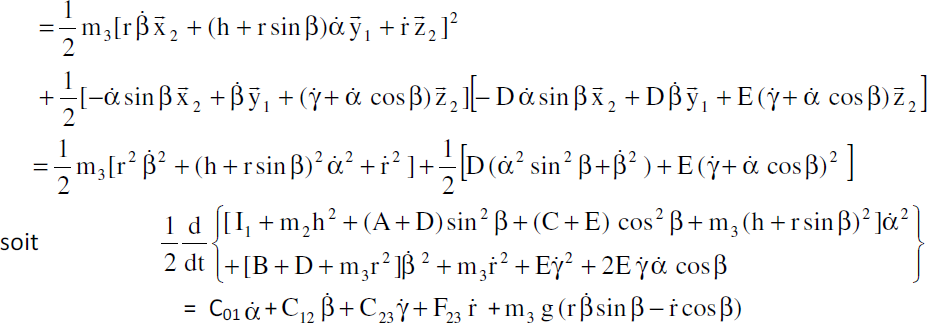
\includegraphics[width=\linewidth]{cor_05}
%\end{center}


